\documentclass[10pt, a4paper, twocolumn]{article}
\usepackage{graphicx}
\usepackage{float}
\usepackage{amsmath}

\usepackage[backend=biber]{biblatex}
\addbibresource{cost-attribution.bib}

\title{Cost Attribution for Multi-cloud / Multi-platform Applications}
\author{Mya Pitzeruse}

\begin{document}
\maketitle

\begin{abstract}
  This paper details a solution to attributing cost across common infrastructure.
  The original target for the solution was a hybrid-cloud infrastructure.
  This led to a comprehensive, yet flexible design.
  As a result, its concepts are generic and support both cloud and non-cloud ecosystems.
  The primary goal is to provide a single pane of glass for the distribution of spend across platforms.
\end{abstract}


\section*{Introduction}
  Products run across a variety of platforms.
  Many use a combination of platforms to perform work efficiently.
  Managed database services allow teams to focus on their application logic.
  Apache Hadoop is popular amongst the data science community for analyzing data.
  Meanwhile, platforms like Kubernetes have gained popularity amongst engineers for orchestrating systems.
  Each of these platforms play a role in the development of a single product.

  \begin{figure}[H]
    \centering
    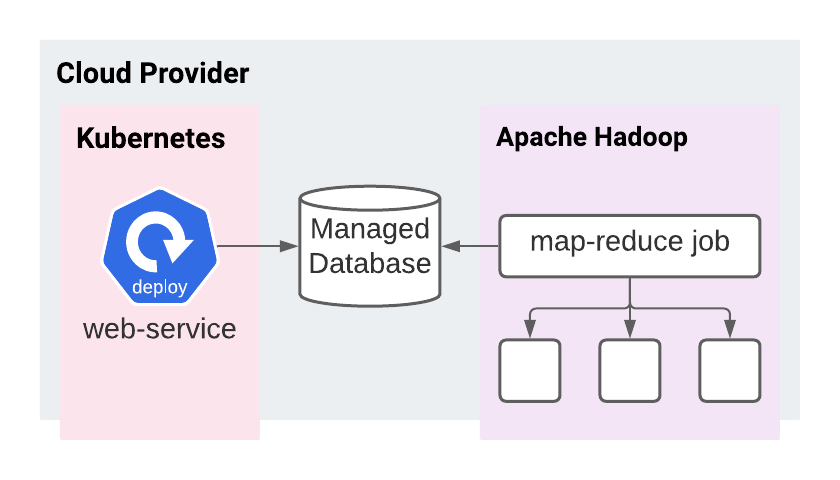
\includegraphics[width=\linewidth]{./cost-attribution-application.png}
    \caption{A multiple platform application}
    \label{figure:1}
  \end{figure}

  Smaller organizations are often less concerned about attributing spend to each product.
  In most cases, these organizations need to know if they're profitable.
  As an organization grows, they often add new products.
  With each new product, this figure grows more complex.
  As a result, the need to attribute spend increases as well.
  Executives often want to know how much each of their products cost.
  This helps determine what their return on investment is.
  When asked, leaders often need to take time to track down this information.

  Solutions like \textit{cloudtamer.io} help organizations better manage their spend on cloud providers ~\cite{cloudtamer}.
  But these solutions often lack visibility into clustered environments.
  You can pair this with in cluster solutions like \textit{kubecost} provide visibility into the cost of Kubernetes pods ~\cite{kubecost}.
  But in the end, you wind up back to where you started.
  Needing to query several sources for information.

  While these account for common cases, it fails to consider less common ones.
  Suppose one part of your organization runs a service on behalf of the rest.
  You might want to apportion usage of that service out to it's heaviest consumers.
  Through the course of my research, I found that no (if not few) comprehensive solutions exist.
  In designing a comprehensive solution, I wanted to ensure compatibility with existing solutions.


\section*{Background}
  In November 2018, Indeed was feeling some pain-points scaling our Apache Mesos infrastructure.
  Some efforts towards a Kubernetes based ecosystem had been underway.

  The first effort focused on a short-term migration.
  It would allow us to move off Apache Mesos while preserving the structure of our ecosystem.
  The second focused on how to run upstream Kubernetes safely and securely.
  As we migrated to Kubernetes, teams built out some cost attribution.
  We wanted to report on changes as teams underwent these migrations.

  We raised similar questions as we began our journey to the the cloud.
  During this time, we considered several solutions.
  Many of them focused on solving in cluster or out of cluster costs, not both.
  When working with several organizations out there, I learned many face similar problems.
  Either they wanted a more comprehensive solution or used several to fill in the gaps.
  At the time, my focus at work was pretty deep into this space.

  In discovering a lack of a comprehensive solutions, I started in on some research.
  I looked to open source to see what solutions did well and what they were missing.
  I looked at the data that was already reported and how that information could be used.
  In doing so, I identified several commonalities across each of them.

  \begin{itemize}
    \item One or more workloads compose a product
    \item Workloads have a unique platform identifier and need resources to run
    \item Resources between each data set varied with some commonality
    \item Each represented an exchange of services between one group and their customers
  \end{itemize}

  These discoveries lead to the design a development of a common reporting platform.
  Designed with decomposition in mind, the platform allows for the addition of layers.
  This allows organizations to start out broad and get more granular over time.


\section*{Concepts}
  This section contains concepts that are fundamental to the solution.
  Understanding them will help map them to potential internal concepts.

  \subsection*{Workloads}
    One or more workloads compose a product
    Workloads represent a variety of processes an organization might run.
    They can be a long running, public facing web services or background jobs.
    Workloads can run across a variety of platforms but are often deployed to one.

  \subsection*{Resources}
    Workloads need resources to run.
    Common cases need things like CPU, memory, and disk.
    At the same time, resources are available through a variety of platforms.
    Kubernetes finds room within the cluster to run containers based on their requests.
    Virtual machines provide a similar allocation of resources, while also providing virtualized hardware.
    Regardless of where and how the workloads run, resources are uniform.

  \subsection*{Standard Units of Measure}
    With anything we measure, standardization and documentation of units is important.
    Without it, one group might code against one standard while another codes using a second.
    Some standardized units of measure include:

    \begin{itemize}
      \item \textbf{CPU} is measured in \textbf{millicores}
      \item \textbf{GPU} is measured in \textbf{cores}
      \item \textbf{Memory} is measured in \textbf{bytes}
      \item \textbf{Disk} is measured in \textbf{bytes} and \textbf{iops}
      \item \textbf{Transport} is measured in \textbf{bytes}
      \item \textbf{Time} is measured in \textbf{milliseconds}
      \item An \textbf{API} is measured in \textbf{requests per second}
      \item \textbf{Energy usage} is measured in \textbf{kilowatt-hours}
    \end{itemize}

    Finer grained units can be used if needed.

  \subsection*{Uniform Resource Names}
    A uniform resource name (URN) is a globally unique, persistent, location-independent identifier ~\cite{rfc8141}.
    While deprecated in 2005, they continue to see use today.
    To help understand URNs a bit more, let's consider an example using RFCs.
    The following URN is for RFC-2141 ~\cite{rfc2141}, the specification for URNs.

\begin{verbatim}
  urn:ietf:rfc:2141
\end{verbatim}

    This URN uses the \textit{ietf} namespace with the \textit{rfc} namespace-specific string.
    To ensure uniqueness, you must register namespaces with the Internet Assigned Numbers Authority (IANA).
    For simplicity, we will use the \textit{workload} namespace.
    This namespace has \textbf{not} been registered and only serves as demonstration.

    A URN in this document refers to specific workloads.
    Let us consider a database deployment MySQL name appdb.
    At some point, you migrate appdb from MySQL to PostgreSQL.
    During this time, both a MySQL and PostgreSQL resource will exist with the name appdb.
    As a result, you should scope your identifiers.
    The block below enumerates several examples of further scoping by class and kind.

\begin{verbatim}
  urn:workload:aws:642135246531
  urn:workload:compute:host:appname
  urn:workload:compute:vm:appname
  urn:workload:compute:pod:appname
  urn:workload:compute:container:appname
  urn:workload:storage:postgres:appdb
  urn:workload:storage:mysql:appdb
  urn:workload:storage:rds:appdb
  urn:workload:storage:aurora:appdb
  urn:workload:storage:spanner:appdb
\end{verbatim}

    \subsubsection*{Amazon's ARN}
      Amazon leverages it's own resource naming scheme called ARNs.
      Like URNs, ARNs represent a unique resource in AWS.
      The solution described herein should support ARNs in place of URNs.
      It's recommended that URNs are consistent for simplicity and ease of use.

  \subsection*{Double-entry Bookkeeping}
    Double-entry bookkeeping is a common practice used by most (if not all) regulated financial systems ~\cite{doubleentry}.
    It is often used to keep accounts balanced and as an error detection tool.
    Implementation of such a system requires several key details:

    \begin{itemize}
      \item Each entry added is immutable.
      \item Every entry added to one account, requires a corresponding entry in the other account.
      \item Independent tracking of charges (debits) and payments (credits).
    \end{itemize}

    Double-entry systems are often implemented as a ledger.
    This allows the system to track transactions for a given account.
    In this solution, we augment the traditional approach to double-entry bookkeeping with hierarchy.
    We do this to model the real-world exchange of resources between groups.
    Consider Figure~\ref{figure:2}.

    \begin{figure}[H]
      \centering
      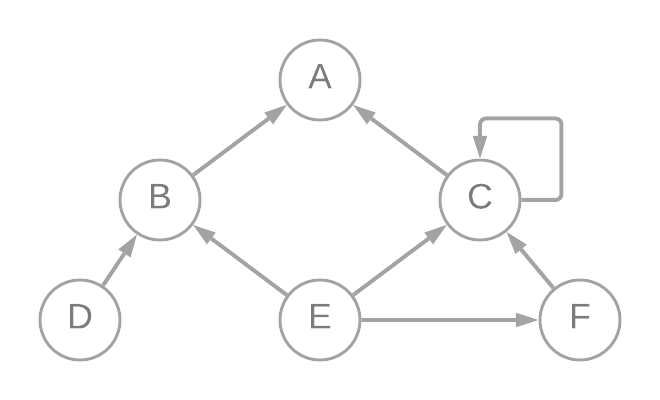
\includegraphics[width=\linewidth]{./cost-attribution-graph.png}
      \caption{Exchange of service graph}
      \label{figure:2}
    \end{figure}

    This graph shows how projects can build upon one another to deliver value to the business.
    For example, E uses services provided by B, C, and F.
    At the end of the day, we want to attribute E the resources that they consume.

\section*{Implementation}
  When it comes to implementation, I've found there are two schools of thought.

  The first approach is to use real world dollars.
  There can be some challenge in this approach.
  If you work for an international organization, you'll need to choose a base currency.
  Then, you'll need to consider things like exchange rates.
  In many ways, this information is valuable for product owners.
  It communicates how much their system costs and helps them determine a price for their service.
  In the wrong hands, this information is dangerous.

  The second approach is to use a basis point type of system.
  This approach allows you to represent the underlying usage as a percentage.
  One problem with this approach is that when you scale a cluster up, usage goes down.
  This can be confusing if you haven't deployed changes recently, but see a shift in your usage.

  At the end of the day, we need a combination of approaches.
  We can use basis points to apportion out usage at each tier.
  When displaying or analyzing information, we can provide a currency value.
  The currency value could be synthetic, an estimate, or a real world value.
  This approach allows for the most accurate representation of a given products cost.

  \subsection*{Apportioning Usage}
    Apportioning usage is the process of dividing a pool of resources amongst its consumers.
    In this solution, we do this using basis points.
    Basis points represent fractional percentages.
    They are often represented as one hundredth of a percent.
    We use basis points as it helps address a couple of challenges.

    \begin{enumerate}
      \item Normalize measurements to a common unit
      \item Better handle cases of over-commit resources
    \end{enumerate}

    To determine basis points for a process, we need to know what the total available resources are.
    The total (\textit{T}) will be the larger of what is \textit{available} (common case) and what is \textit{reserved} (over-commit).
    We apply the process to each resource we want to apportion out.
    The equations below compute the total availability of a given resource.

    \begin{gather*}
      T_{reserved} = \sum^{workloads}_{W} max(W_{reserved}, W_{usage}) \\
      \\
      T = max(T_{available}, T_{reserved}) \\
    \end{gather*}

    Once you've computed the total amount of a resource, you can distribute basis points.
    The equation below calculate basis points for a single resource for a single workload.

    \begin{gather*}
      basispoints = \frac{max(reserved, usage)}{T} * 100 \\
    \end{gather*}

    At the end, we have a set of basis points for each resource we want to charge for.
    We need to convert this set of basis points to a single basis point.
    A simple approach would be to take the average.
    Taking an average of percentages requires some care ~\cite{indeed,robertoreif}.
    In this case, we can take steps to ensure taking an average of percentages is safe and representative of the underlying usage.

    We should keep in mind that these basis points are being distributed at each node in our graph.
    This ensures that we know the full scope of data at the time we calculate percentages.
    This also ensures that the sample size of the data is the same for each resource we calculate.
    This means that we compute basis points from a constant or a computed value from the same record set.
    Because of this, we can safely leverage an average of basis points.
    Let us consider the following allocations.

    \begin{itemize}
      \item \textbf{10000} basis points from GPU reservations
      \item \textbf{1000} basis points from CPU reservations
      \item \textbf{3000} basis points from memory reservations
    \end{itemize}

    The above workload averages out with \textbf{4667} basis points.
    Suppose this workload ran in a shared cluster with one other workload.
    That workload claims the remaining resources (0 GPU, 9000 CPU, 7000 memory) which averages \textbf{5333} basis points.
    Together, they sum to \textbf{10000} or 100\%.
    This will allow us to annotate every edge with a single weight.

    \begin{figure}[H]
      \centering
      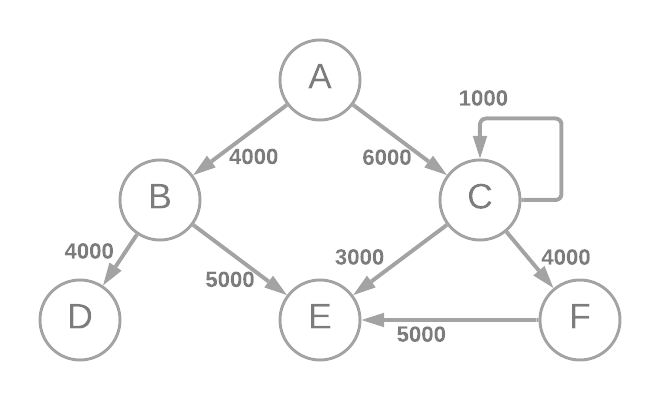
\includegraphics[width=\linewidth]{./cost-attribution-graph-weighted.png}
      \caption{Weighted exchange of service graph}
      \label{figure:3}
    \end{figure}

    In a properly weighted graph, the sum of all weights for a node should be less than or equal to \textbf{10000}.

    \[ 10000 \leq \sum_{edge}^{node} edge_{weight} \]

  \subsection*{Apportioning Cost}
    As said earlier, apportioning usage is not enough.
    There needs to be able to be a monetary value.
    Now, this monetary value could be a real value, like a bill.
    Or, it could be a synthetic value that someone made up.

    It works by attaching a cost to a root workload in the graph.
    From there, we can derive all subsequent charges using common, well known algorithms.

    \subsubsection*{Path Enumeration}
      In most cases, we want to know the cost of a single product.
      Path enumeration provides a list of all paths between a pair of vertices in a graph ~\cite{Grossi2016}.
      We can apply this same concept using a single starting vertex and a direction to search.
      The following is a path enumeration for \textit{A} in Figure~\ref{figure:3}.

      \begin{enumerate}
        \item A, B, D
        \item A, B, E
        \item A, C, E
        \item A, C, F, E
      \end{enumerate}

      Similarly, we can apply this in the opposite direction.
      The following is an inverse path enumeration for \textit{E}.

      \begin{enumerate}
        \item E, B, A
        \item E, C, A
        \item E, F, C, A
      \end{enumerate}

      This process is key to attributing cost.

    \subsubsection*{Computing Cost}
      Using the enumerated paths, we can compute the total cost for a given workload.
      We compute costs using the weights on the edge of the graph in combination with root costs.
      The equations are as follows.

      \begin{gather*}
        \forall^{workloads}_{w} \\
        \\
        cost(w) = \sum^{paths}_{p} cost(p) \\
        \\
        cost(p) = root(p) \times \prod^{p}_{edge} (weight / 10000) \\
        \\
        root(p) = p[len(p) - 1]_{cost} \\
      \end{gather*}

      To help explain, let's consider \textit{D}.
      It has a single path, \textit{D, B, A}.
      Figure~\ref{figure:4} highlights this path in blue.

      \begin{figure}[H]
        \centering
        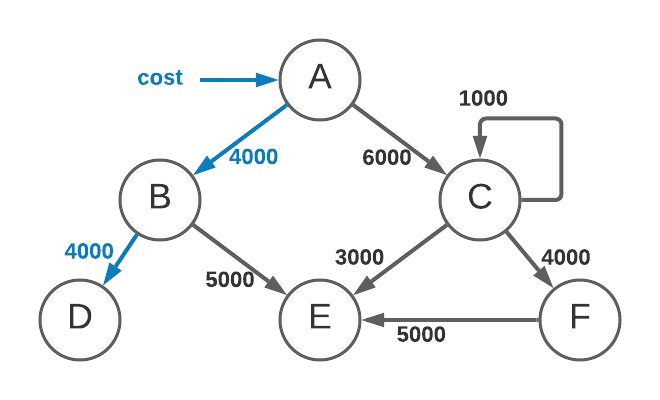
\includegraphics[width=\linewidth]{./cost-attribution-cost-d.png}
        \caption{p1 for D}
        \label{figure:4}
      \end{figure}

      Using the information in the graph and our equations, we can compute a cost for \textit{D}.

      \begin{gather*}
        cost(p_{1}) = A_{cost} \times 0.4 \times 0.4 \\
        \\
        cost(D) = A_{cost} \times 0.16 \\
      \end{gather*}

      If \textit{A} costs \textbf{100 USD}, then \textit{D} costs \textbf{16 USD}.
      Similarly, we can consider a more complicated example.
      \textit{E} has three paths.
      They are documented in the section on Path Enumeration and
      highlighted in Figures~\ref{figure:5},~\ref{figure:6},~and~\ref{figure:7}.

      \begin{figure}[H]
        \centering
        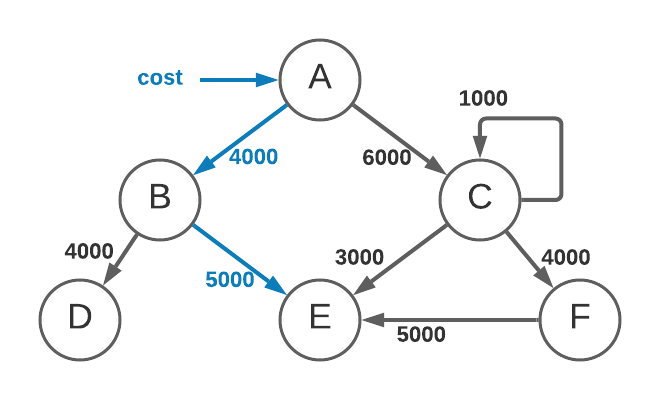
\includegraphics[width=\linewidth]{./cost-attribution-cost-ep1.png}
        \caption{p1 for E}
        \label{figure:5}
      \end{figure}

      \begin{figure}[H]
        \centering
        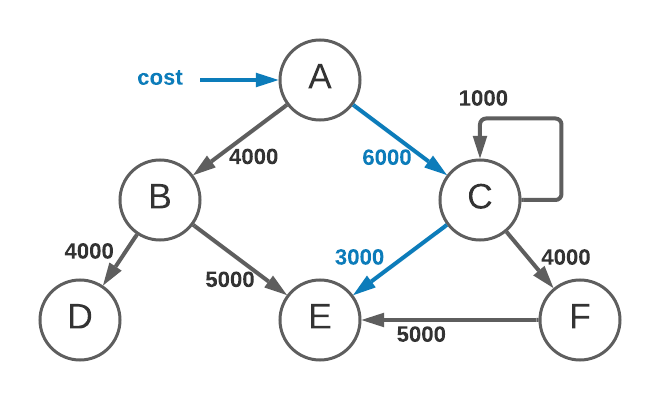
\includegraphics[width=\linewidth]{./cost-attribution-cost-ep2.png}
        \caption{p2 for E}
        \label{figure:6}
      \end{figure}

      \begin{figure}[H]
        \centering
        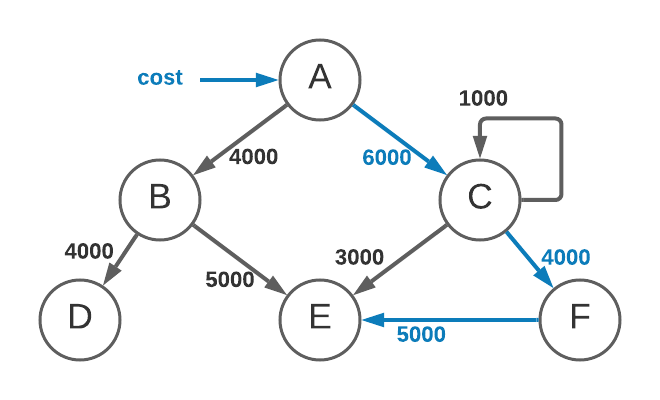
\includegraphics[width=\linewidth]{./cost-attribution-cost-ep3.png}
        \caption{p3 for E}
        \label{figure:7}
      \end{figure}

      While more complicated, the process is the same.

      \begin{gather*}
        cost(p_{1}) = A_{cost} \times 0.4 \times 0.5 \\
        cost(p_{2}) = A_{cost} \times 0.6 \times 0.3 \\
        cost(p_{3}) = A_{cost} \times 0.6 \times 0.4 \times 0.5 \\
        \\
        cost(E) = A_{cost} \times (0.2 + 0.18 + 0.12) \\
        cost(E) = A_{cost} \times 0.5 \\
      \end{gather*}

      If \textit{A} costs \textbf{100 USD}, then \textit{E} costs \textbf{50 USD}.

  \subsection*{Reconciling Cost}
    As we are dealing with a financial system, we should ensure we apportion cost correctly.
    In accounting, we use reconciliation to ensure that money leaving an account matches the actual money spent.
    We can use the same process to balance our computed costs against the provided costs.
    Table~\ref{table:1} demonstrates how we balance and reconcile accounts.

    \begin{table}[H]
      \centering
      \begin{tabular}{ l|c|r|c }
        $w$ & Spend            & Attributed & Balance           \\
        \hline
        A   & $ x            $ &      10000 & $ 0             $ \\
        B   & $ x \times .4  $ &       9000 & $ x \times 0.04 $ \\
        C   & $ x \times .6  $ &       7000 & $ x \times 0.18 $ \\
        D   & $ x \times .16 $ &          0 & $ x \times 0.16 $ \\
        E   & $ x \times .5  $ &          0 & $ x \times 0.50 $ \\
        F   & $ x \times .24 $ &       5000 & $ x \times 0.12 $ \\
        \hline
            &                  &            & $ x \times 1.00 $ \\
      \end{tabular}
      \caption{Reconciliation}
      \label{table:1}
    \end{table}

    We compute this using the current spend and the current attributed amount.
    The attributed amount shouldn't factor in anything attributed back to your own team.
    Using the following equation, we compute the remaining balance for each item.

    \[ balance(w) = spend \times \left(1 - \frac{attributed}{10000}\right) \]

    To help solidify this, let us consider the  example from earlier.
    If \textit{A} cost \textbf{100 USD}, the balance for each would be as follows.

    \begin{table}[H]
      \centering
      \begin{tabular}{ l|c|r }
        $w$ & Balance & USD \\
        \hline
        A   & $ 0             $ & $\$0$   \\
        B   & $ x \times 0.04 $ & $\$4$   \\
        C   & $ x \times 0.18 $ & $\$18$  \\
        D   & $ x \times 0.16 $ & $\$16$  \\
        E   & $ x \times 0.50 $ & $\$50$  \\
        F   & $ x \times 0.12 $ & $\$12$  \\
        \hline
            & $ x \times 1.00 $ & $\$100$ \\
      \end{tabular}
      \caption{Balance Sheet}
      \label{table:2}
    \end{table}

    This shows that the approach to cost attribution described herein balances.

  \subsection*{The Ledger}
    Accountants leverage ledgers to track transactions between two parties.
    Consider Table~\ref{table:2} and Table~\ref{table:3}.
    They detail the fields and data types of the ledger.
    Each entry in the ledger represents a workload specified by a URN.

    \begin{table}[H]
      \centering
      \begin{tabular}{ l|l }
        Field & Explanation \\
        \hline
        datetime & Time of transaction \\
        payer & Who received services (from) \\
        payee & Who provides services (to) \\
        type & A debit or credit \\
        usage & The usage \\
        urn & A uniform resource name \\
        detail & A break down of charges \\
        labels & Organization specific metadata \\
      \end{tabular}
      \caption{Fields}
      \label{table:3}
    \end{table}

    \begin{table}[H]
      \centering
      \begin{tabular}{ l|l }
        Field & Type \\
        \hline
        datetime & datetime, int64 \\
        payer & string \\
        payee & string \\
        type & enum(debit, credit) \\
        usage & int32 \\
        urn & string \\
        detail & map[string]int32 \\
        labels & map[string]string \\
      \end{tabular}
      \caption{Field types}
      \label{table:4}
    \end{table}

    Usage can store basis points or a monetary value.
    Storing data as basis points make it quick and easy to record allocations over time.
    We can later compute a monetary ledger using the basis point one and a set of bills.

\section*{Parting Thoughts}
  \subsection*{Importance of Modeling}
    Data modeling plays a major role in proper representation of resource consumption.
    While it's easy to apportion resources at a cluster level, it often misses nuances.
    For example, CPU heavy nodes or GPU nodes cost more than common compute.
    As a result, resources may be weighted allowing preferential distribution of cost.
    With proper data modeling you ensure the cost of those nodes are apportioned properly.

  \subsection*{Data Storage}
    The ledger can take many shapes and forms.
    Storage should use a consistent system.
    Eventually consistent systems can leave you in troublesome positions when reconciling cost.
    Indexing labels on the ledger allows for the categorization of edge data.
    The enabled further analysis and grouping into hierarchies, such as your organization structure.

  \subsection*{Multiple Roots}
    Throughout this document, we've demonstrated the process using a single product with a cost.
    In practice, this graph is often more complex than that.
    Regardless, the process is still the same.

  \subsection*{Equitable Distribution}
    In some cases, products may not distribute all their resources amongst their consumers.
    This often leaves them with an overhead that they are responsible for.
    In this case, groups may choose to re-distribute their overhead amongst their consumers.
    This process is often referred to as equitable distribution.
    The following equation computes a redistribution value to distribute amongst your customers.

    \[ redistribution = \frac{10000 - billable}{consumers} \]

\printbibliography

\end{document}
